%Dokumentklasse
\documentclass{alex_bericht}
%\usepackage[onehalfspacing]{setspace}
% ============= Packages =============

% Dokumentinformationen



% Standard Packagesa
%\usepackage{fancyhdry}
\graphicspath{{img/}}
\usepackage{lmodern}
\usepackage{color}

% zusätzliche Schriftzeichen der American Mathematical Society


%nicht einrücken nach Absatz
%\setlength{\parindent}{0pt}


% ============= Kopf- und Fußzeile =============
%\pagestyle{fancy}
%
%\lhead{}
%\chead{}
%\rhead{\slshape \leftmark}
%%%
%\lfoot{}
%\cfoot{\thepage}
%\rfoot{}
%%
%\renewcommand{\headrulewidth}{0.4pt}
%\renewcommand{\footrulewidth}{0pt}

% ============= Package Einstellungen & Sonstiges ============= 
%Besondere Trennungen
\hyphenation{De-zi-mal-tren-nung}


% ============= Dokumentbeginn =============

\begin{document}
%Seiten ohne Kopf- und Fußzeile sowie Seitenzahl
\pagestyle{empty}
\pagenumbering{Roman}

\titlehead{
\includegraphics[width=5cm]{logo.jpg}}
\title{Einfacher harmonischer Oszillator}
\author{Alexander Helbok\thanks{\href{mailto:alexander.helbok@student.uibk.ac.at}{alexander.helbok@student.uibk.ac.at}}, Clemens Bein\thanks{\href{mailto:clemens.bein@uibk.ac.at}{clemens.bein@uibk.ac.at}}}
\date{\today}
\maketitle
\vfill 


\clearpairofpagestyles
\pagestyle{headings}
% !TeX root = 00_Vorlage.tex
% !TeX spellcheck = de_DE
\addsec{Zusammenfassung}
\label{sec:zusammenfassung}


Ziel dieses Versuches ist es, ein Modell aufzustellen, welches die Federkonstante $k$ eines Systems paralleler Federn zu vorhersagt. Dies erfolgt in drei Versuchen. Im Ersten wird die Federkonstante von einer Feder mit Hilfe drei verschiedener Massen bestimmt, daraufhin wird im zweiten Versuch die Federkonstante von zwei parallelen Federn bestimmt und dem ersten Versuch gegenübergestellt. Aus diesem Vergleich wird nun ein erstes Modell entwickelt, mit welchen man die Federkonstante $k$ für ein System aus $N$ parallelen Feder berechnen kann. Im letzten Versuch wird nun dieses Modell, mit Hilfe von einem System mit drei parallelen Federn, geprüft. Im gesamten wurde das Modell angenommen, dadurch folgt das die Versuchsreihe erfolgreich war.


% Beendet eine Seite und erzwingt auf den nachfolgenden Seiten die Ausgabe aller Gleitobjekte (z.B. Abbildungen), die bislang definiert, aber noch nicht ausgegeben wurden. Dieser Befehl fügt, falls nötig, eine leere Seite ein, sodaß die nächste Seite nach den Gleitobjekten eine ungerade Seitennummer hat. 
\cleardoubleoddpage

% pagestyle für gesamtes Dokument aktivieren
%\pagestyle{fancy}

%Inhaltsverzeichnis
\tableofcontents

%Verzeichnis aller Bilder
\listoffigures

%Verzeichnis aller Tabellen
\listoftables
\cleardoubleoddpage

\pagenumbering{arabic}
% !TeX root = 00_Vorlage.tex
% !TeX spellcheck = de_DE
\chapter{Einleitung}
\label{sec:einleitung}

Harmonische Oszillationen sind nicht nur, wie in diesem Versuch, in der Mechanik anzutreffen, sondern erstreckt sich von der Elektrodynamik bis hin zur Quantenmechanik über alle Teilbereiche der Physik. Das aus der analytischen Mechanik abgeleitete Modell des harmonischen Oszillators eignet sich auch gut, um nicht-mechanische Konzepte zu beschreiben und anzunähern, wie zum Beispiel die Bindungsenergien von Atomen. Es wird nicht umsonst gescherzt, dass sich alles zu einem harmonischen Oszillator reduziert. Mit so vielen Anwendungen ist die physikalische Beschreibung des harmonischen Oszillator eine der wichtigsten Werkzeuge der Physik. Dadurch ist es lohnenswert, im Grundpraktikum eines dieser Modelle mit Hilfe eines Experimentes zu validieren. Hier wenden wir das Modell des einfachen harmonischen Oszillators auf das Federpendel an.

Dafür werden in \autoref{sec:theorie} die benötigten physikalischen und statistischen Grundlagen aufgezeigt. Daraufhin wird in \autoref{sec:aufbau} der Aufbau und die Vorgehensweise der einzelnen Versuche beschrieben. Insbesondere wird auf die Massenbestimmung, die Berechnung der Federkonstante $k$, das Aufstellen eines Modells und anschließend auf die Überprüfung dieses Modells eingegangen. In \autoref{sec:ergebnisse} werden die Ergebnisse der drei Versuche dargestellt und mit der Theorie verglichen und zum Schluss werden die gewonnen Erkenntnisse diskutiert.


\chapter{Theorie}
\label{sec:grundlagen}


\section{Beispielkapitel}
\label{sec:beispiel}
\begin{figure}[htb]
  \centering  
  
\includegraphics[scale=0.5]{starwars.jpg}
  \caption{Star Wars Logo}
  \label{fig:starwars}
\end{figure}
Weit hinten, hinter den Wortbergen, fern der Länder Vokalien und Konsonantien leben die Blindtexte (siehe Abb \ref{fig:starwars}). Abgeschieden wohnen Sie in Buchstabhausen an der Küste des Semantik, eines großen Sprachozeans. Ein kleines Bächlein namens Duden fließt durch ihren Ort und versorgt sie mit den nötigen Regelialien. Es ist ein paradiesmatisches Land, in dem einem gebratene Satzteile in den Mund fliegen. Nicht einmal von der allmächtigen Interpunktion werden die Blindtexte beherrscht – ein geradezu unorthographisches Leben. Eines Tages aber beschloß eine kleine Zeile Blindtext, ihr Name war Lorem Ipsum, hinaus zu gehen in die weite Grammatik. Der große Oxmox riet ihr davon ab, da \cite{test}.
Weit hinten, hinter den Wortbergen, fern der Länder Vokalien und Konsonantien leben die Blindtexte (siehe Abb \ref{fig:starwars}). Abgeschieden wohnen Sie in Buchstabhausen an der Küste des Semantik, eines großen Sprachozeans. Ein kleines Bächlein namens Duden fließt durch ihren Ort und versorgt sie mit den nötigen Regelialien. Es ist ein paradiesmatisches Land, in dem einem gebratene Satzteile in den Mund fliegen. Nicht einmal von der allmächtigen Interpunktion werden die Blindtexte beherrscht – ein geradezu unorthographisches Leben. Eines Tages aber beschloß eine kleine Zeile Blindtext, ihr Name war Lorem Ipsum, hinaus zu gehen in die weite Grammatik.

Weit hinten, hinter den Wortbergen, fern der Länder Vokalien und Konsonantien leben die Blindtexte (siehe Abb \ref{fig:starwars}). Abgeschieden wohnen Sie in Buchstabhausen an der Küste des Semantik, eines großen Sprachozeans. Ein kleines Bächlein namens Duden fließt durch ihren Ort und versorgt sie mit den nötigen Regelialien. Es ist ein paradiesmatisches Land, in dem einem gebratene Satzteile in den Mund fliegen. Nicht einmal von der allmächtigen Interpunktion werden die Blindtexte beherrscht – ein geradezu unorthographisches Leben. Eines Tages aber beschloß eine kleine Zeile Blindtext, ihr Name war Lorem Ipsum, hinaus zu gehen in die weite Grammatik.
Weit hinten, hinter den Wortbergen, fern der Länder Vokalien und Konsonantien leben die Blindtexte (siehe Abb \ref{fig:starwars}). Abgeschieden wohnen Sie in Buchstabhausen an der Küste des Semantik, eines großen Sprachozeans. Ein kleines Bächlein namens Duden fließt durch ihren Ort und versorgt sie mit den nötigen Regelialien. Es ist ein paradiesmatisches Land, in dem einem gebratene Satzteile in den Mund fliegen. Nicht einmal von der allmächtigen Interpunktion werden die Blindtexte beherrscht – ein geradezu unorthographisches Leben. Eines Tages aber beschloß eine kleine Zeile Blindtext, ihr Name war Lorem Ipsum, hinaus zu gehen in die weite Grammatik.

Weit hinten, hinter den Wortbergen, fern der Länder Vokalien und Konsonantien leben die Blindtexte (siehe Abb \ref{fig:starwars}). Abgeschieden wohnen Sie in Buchstabhausen an der Küste des Semantik, eines großen Sprachozeans. Ein kleines Bächlein namens Duden fließt durch ihren Ort und versorgt sie mit den nötigen Regelialien. Es ist ein paradiesmatisches Land, in dem einem gebratene Satzteile in den Mund fliegen. Nicht einmal von der allmächtigen Interpunktion werden die Blindtexte beherrscht – ein geradezu unorthographisches Leben. Eines Tages aber beschloß eine kleine Zeile Blindtext, ihr Name war Lorem Ipsum, hinaus zu gehen in die weite Grammatik.
Weit hinten, hinter den Wortbergen, fern der Länder Vokalien und Konsonantien leben die Blindtexte (siehe Abb \ref{fig:starwars}). Abgeschieden wohnen Sie in Buchstabhausen an der Küste des Semantik, eines großen Sprachozeans. Ein kleines Bächlein namens Duden fließt durch ihren Ort und versorgt sie mit den nötigen Regelialien. Es ist ein paradiesmatisches Land, in dem einem gebratene Satzteile in den Mund fliegen. Nicht einmal von der allmächtigen Interpunktion werden die Blindtexte beherrscht – ein geradezu unorthographisches Leben. Eines Tages aber beschloß eine kleine Zeile Blindtext, ihr Name war Lorem Ipsum, hinaus zu gehen in die weite Grammatik.

Weit hinten, hinter den Wortbergen, fern der Länder Vokalien und Konsonantien leben die Blindtexte (siehe Abb \ref{fig:starwars}). Abgeschieden wohnen Sie in Buchstabhausen an der Küste des Semantik, eines großen Sprachozeans. Ein kleines Bächlein namens Duden fließt durch ihren Ort und versorgt sie mit den nötigen Regelialien. Es ist ein paradiesmatisches Land, in dem einem gebratene Satzteile in den Mund fliegen. Nicht einmal von der allmächtigen Interpunktion werden die Blindtexte beherrscht – ein geradezu unorthographisches Leben. Eines Tages aber beschloß eine kleine Zeile Blindtext, ihr Name war Lorem Ipsum, hinaus zu gehen in die weite Grammatik.
Weit hinten, hinter den Wortbergen, fern der Länder Vokalien und Konsonantien leben die Blindtexte (siehe Abb \ref{fig:starwars}). Abgeschieden wohnen Sie in Buchstabhausen an der Küste des Semantik, eines großen Sprachozeans. Ein kleines Bächlein namens Duden fließt durch ihren Ort und versorgt sie mit den nötigen Regelialien. Es ist ein paradiesmatisches Land, in dem einem gebratene Satzteile in den Mund fliegen. Nicht einmal von der allmächtigen Interpunktion werden die Blindtexte beherrscht – ein geradezu unorthographisches Leben. Eines Tages aber beschloß eine kleine Zeile Blindtext, ihr Name war Lorem Ipsum, hinaus zu gehen in die weite Grammatik.


\section{Beispielunterkapitel}
\label{subsec:beispiel}

Weit hinten, hinter den Wortbergen, fern der Länder Vokalien und Konsonantien leben die Blindtexte (siehe Abb \ref{fig:starwars}). Abgeschieden wohnen Sie in Buchstabhausen an der Küste des Semantik, eines großen Sprachozeans. Ein kleines Bächlein namens Duden fließt durch ihren Ort und versorgt sie mit den nötigen Regelialien. Es ist ein paradiesmatisches Land, in dem einem gebratene Satzteile in den Mund fliegen. Nicht einmal von der allmächtigen Interpunktion werden die Blindtexte beherrscht – ein geradezu unorthographisches Leben. Eines Tages aber beschloß eine kleine Zeile Blindtext, ihr Name war Lorem Ipsum, hinaus zu gehen in die weite Grammatik.
Weit hinten, hinter den Wortbergen, fern der Länder Vokalien und Konsonantien leben die Blindtexte (siehe Abb \ref{fig:starwars}). Abgeschieden wohnen Sie in Buchstabhausen an der Küste des Semantik, eines großen Sprachozeans. Ein kleines Bächlein namens Duden fließt durch ihren Ort und versorgt sie mit den nötigen Regelialien. Es ist ein paradiesmatisches Land, in dem einem gebratene Satzteile in den Mund fliegen. Nicht einmal von der allmächtigen Interpunktion werden die Blindtexte beherrscht – ein geradezu unorthographisches Leben. Eines Tages aber beschloß eine kleine Zeile Blindtext, ihr Name war Lorem Ipsum, hinaus zu gehen in die weite Grammatik.

% !TeX root = 00_Vorlage.tex
% !TeX spellcheck = de_DE

\chapter{Aufbau und Methoden}
\label{sec:aufbau}
In diesem Kapitel wird der Aufbau der drei Einzelversuche erläutert.
\section{Eine Feder mit drei Massen}
Für diesen Versuch wird eine Feder mit jeweils drei verschiedenen Massen $m_i$ in Schwingung versetzt um aus der Schwingperiode die Federkonstante $k$ zu berechnen. Um drei Verschiedene Massen zu erhalten wird der Versuch einmal nur mit dem IOLab durchgeführt. Für den zweiten Durchgang wird ein Stein mit Klebeband an dem IOLab befestigt und für den dritten Durchgang ein weiterer Stein. Ebenfalls benötigt man eine Feder, das IOLab an dem eine Ringschraube an dem Kraftsensor angebracht ist und eine Briefklammer, welche an einer Stuhllehne befestigt ist.
\subsection{Bestimmung der Masse}
Um nun die einzelnen Massen $m_i$ zu bestimmen wird das IOLab an dem Kraftsensor mit einer Schnur, an einem Fixpunkt aufgehängt. (Siehe \autoref{fig:Massenbestimmung}). Dies wird nun für die zwei weiteren Massen wiederholt. Aus den Daten des Beschleunigungs- und Kraftsensors lässt sich nun die jeweilige Masse bestimmen. 
\begin{figure}[H]
	\centering
	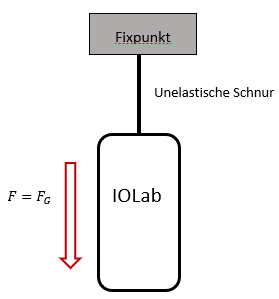
\includegraphics{Massebestimmung}
	\caption[Versuchsaufbau der Massebestimmung]{Schematischer Versuchsaufbau zur Bestimmung der Masse}
	\label{fig:Massenbestimmung}
\end{figure}
\subsection{Bestimmung der Periodendauer}
Nun wird das IOLab an eine Feder statt einer Schnur an dem Kraftsensor und Fixpunkt befestigt und aus dem Ruhepunkt ausgelenkt. Währenddessen wird die Kraft $F$ die auf den Kraftsensor wirkt und die Beschleunigung $a$ aufgezeichnet. Man erhält einen Sinus-artigen Verlauf in beiden Messungen, aus welchen man die Schwingungsperiode auslesen kann. In dem Man die Zeit zwischen fünf Maxima durch vierteilt.
\begin{figure}[H]
	\centering
	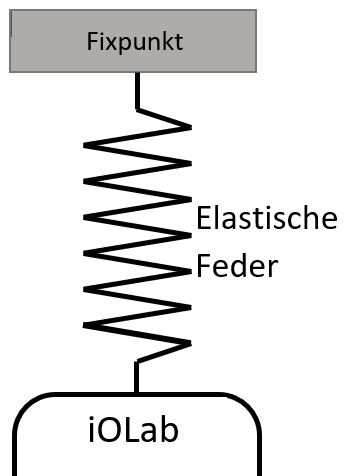
\includegraphics[width=5cm,keepaspectratio]{Schwingung 1}
	\caption[Versuchsaufbau für eine Feder]{Schematische Darstellung des Versuchsaufbau zur Bestimmung der Schwingungsperiode}
	\label{fig:Schwingungsperiode1}
\end{figure}
\subsection{Berechnung der Federkonstante \( k \)}
Wie in Kapitel \autoref{sec:theorie} diskutiert lässt sich nun der Wert für $k$ durch die Schwingungsperiode und der Masse $m_i$ bestimmen.
\section{Aufstellen eines Modells für parallele Federn}
\label{sec:Modell}
Zur Bestimmung eines Modells für die Federkonstante $k$ wird der Versuch mit der schwersten  Masse $m_3$ und zwei parallelen Federn wiederholt. Dazu werden mit Hilfe von zwei Kartonstücken parallel aufgehängt. Die Kartonstücke werden mit einer Büroklammer an dem Kraftsensor und dem Fixpunkt befestigt, wie \autoref{fig:2,3 Federn} zeigt. Anschließend wird das IOLab aus dem Ruhepunkt ausgelenkt und für $20s$ die Kraft $F$ und die Beschleunigung $a$ aufgezeichnet.
\begin{figure}[H]
	\centering
	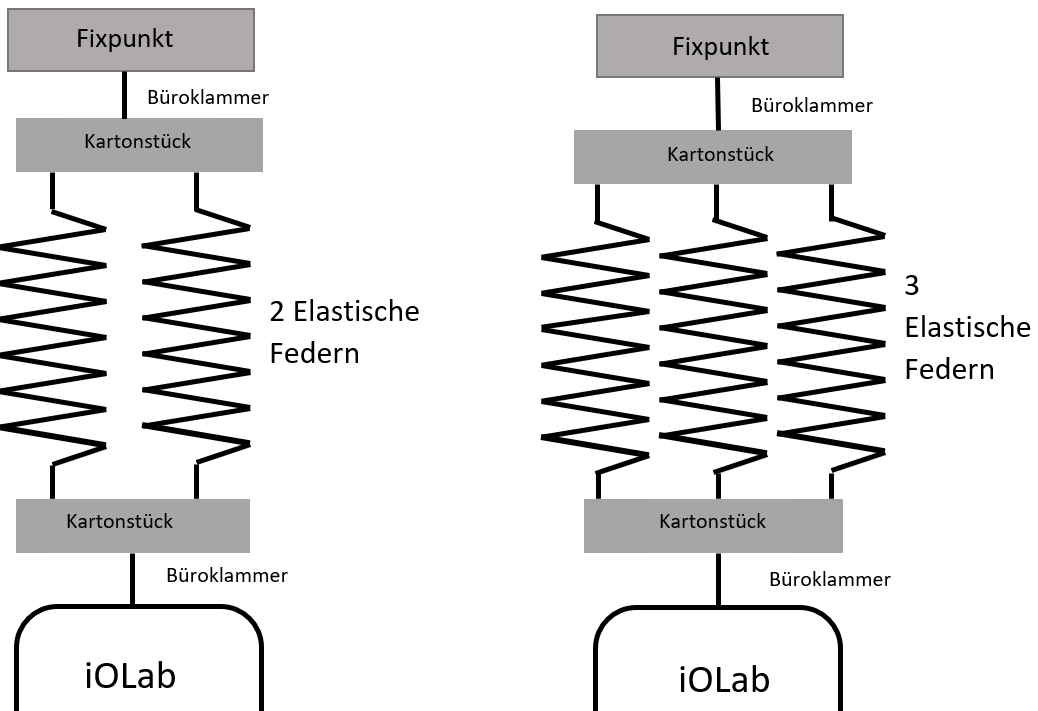
\includegraphics[width=10cm, keepaspectratio]{2,3Federn}
	\caption[Versuchsaufbau mit mehrere Federn]{Schematischer Versuchsaufbau von zwei parallelen Federn(links) und drei Federn (rechts), zur Bestimmung der Periodendauer}
	\label{fig:2,3 Federn}
\end{figure}
Aus dem Vergleich der Federkonstanten $k_1$ und $k_2$ aus \autoref{sec:Modell} lässt sich nun ein Modell für $N$ Federn aufstellen.
\section{Prüfen des Modells}
Um nun das Modell zu überprüfen, erweitern wir obigen Versuch auf parallelen Federn mit selbiger Masse $m_3$ (Siehe \autoref{fig:2,3 Federn}). Bei der Durchführung dieses Versuches muss auf die anfängliche Auslenkung geachtet werden, da es zu Überdehnung der Federn kommen kann und das System dann nicht mehr durch einen harmonischen Oszillator beschrieben wird. Anschließend wird wie im vorherigen Versuch die Federkonstante \( k_3 \) ausgerechnet und mit dem Modell abgeglichen.

% !TeX root = 00_Vorlage.tex
% !TeX spellcheck = de_DE
\chapter{Ergebnisse}
\label{sec:ergebnisse}

Im folgenden Abschnitt werden die Ergebnisse der Massenbestimmungen und der anschließenden Versuchen mit einer und mehrerer Federn. Alle Fehlerangaben beziehen sich auf statistische Fehler; Systematische werden gegebenenfalls separat diskutiert. 

\section{Massenbestimmung}
Die Masse des Pendelkörpers wurde über eine simultane Kraft- und Beschleunigungsmessung und Newtons Axiom \autoref{eqn:newt} bestimmt. In \autoref{fig:mass} sind die Messdaten auf die Zeit aufgetragen. In der ersten halben Sekunde befindet sich das Gerät am Tisch in Ruhe und ab \( t = 4 \unit{s} \) ist das IOLab komplett in der Luft. Ab diesem Zeitpunkt wird eine Konstante an die Messdaten angepasst. 

\begin{figure}[H]
	\centering
	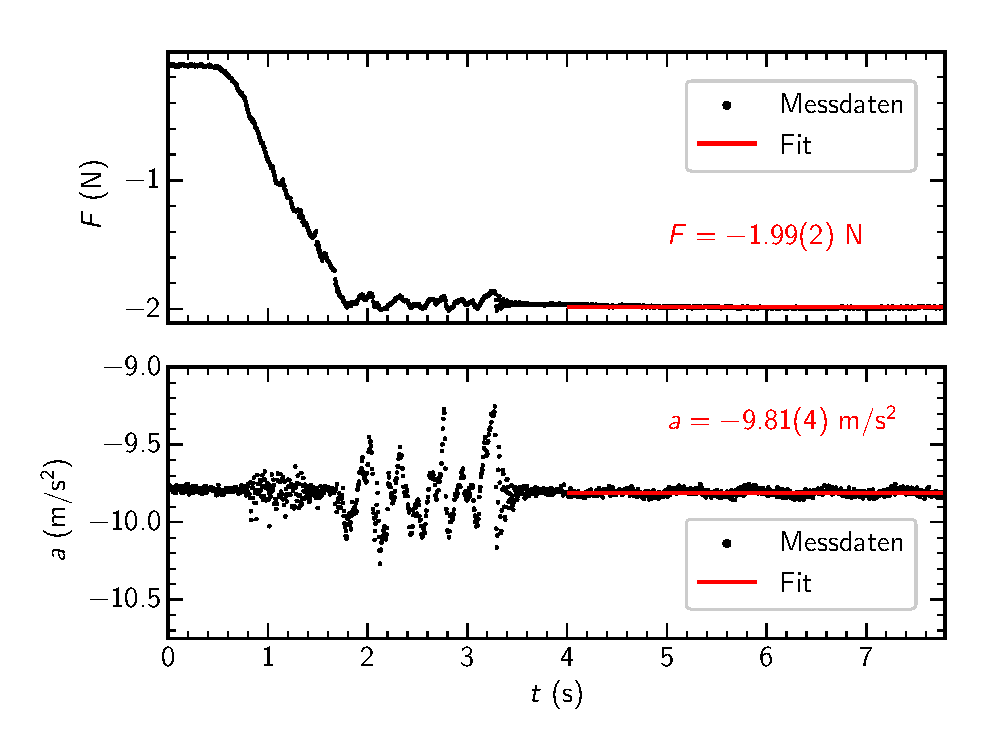
\includegraphics[width=\textwidth]{mass.eps}
	\caption[Bestimmung der Masse]{Vom oben nach unten sind Kraft \( F \) und Beschleunigung \( a \) aufgetragen. Die Fehlerbalken der Daten sind zu klein, um sie auszumachen und werden daher nicht eingetragen. Die zwei Grafiken teilen sich die horizontale Achse. Zudem sind in Rot Geraden von \( t = 4 \unit{s} \) bis \( t = 8 \unit{s} \) angepasst.}
	\label{fig:mass}
\end{figure}

Der bestimmte Wert mit Fehler ist sowohl in der Abbildung, als auch in \autoref{table:1} zu sehen. Die Unsicherheit wurde auf die Standardabweichung der Daten gesetzt, da dann (per Definition) Zwei Drittel der Daten innerhalb des \( 1\sigma \) Intervalls liegen.

\begin{center}
	\captionaboveof{table}[Messdaten zur Massenbestimmung]{Gemessene Beschleunigung und Kraft und die daraus errechnete Masse der drei Versuche.}
	\begin{tabular}{@{\extracolsep{5mm}} 
			r
			S[table-format=1.2(1)]
			S[table-format=1.2(1)]
			S[table-format=1.2(1)]
		}
		\toprule
		\makecell[t]{}
		&   {\makecell[t]{Versuch 1}}
		&   {\makecell[t]{Versuch 2}}
		&   {\makecell[t]{Versuch 3}}\\
		\midrule
		\( a \unit{(\a)} \) & -9.81(4) & -9.73(6) & -9.81(8) \\
		\( F  \unit{(N)} \) & -1.99(2) & -2.78(2) & -3.93(7) \\
		\( m \unit{(kg)} \) & 0.202(2) & 0.286(3) & 0.400(7) \\
		\bottomrule
	\end{tabular}
	\label{table:1}
\end{center}

\section{Federpendel 1}
Für die Analyse der Oszillation wurde der Beschleunigungssensor verwendet, da dieser eine höhere Auflösung als der Kraftsensor besitzt. In \autoref{fig:sine} sind die Schwingungsdaten der zweiten Masse dargestellt. Links sind die ersten fünf Sekunden, in welchen „schöne” Schwingungen auftreten, zu sehen, während rechts die letzten Sekunden der Messung aufgetragen sind. In rot wurde eine Sinuskurve der Form \( f(x) = A\sin(\omega x + \phi) + d \) an die gesamten Messdaten von \( t = 4 \unit{s} \) bis \( t = 27 \unit{s} \) angepasst. 
	
\begin{figure}[H]
	\centering
	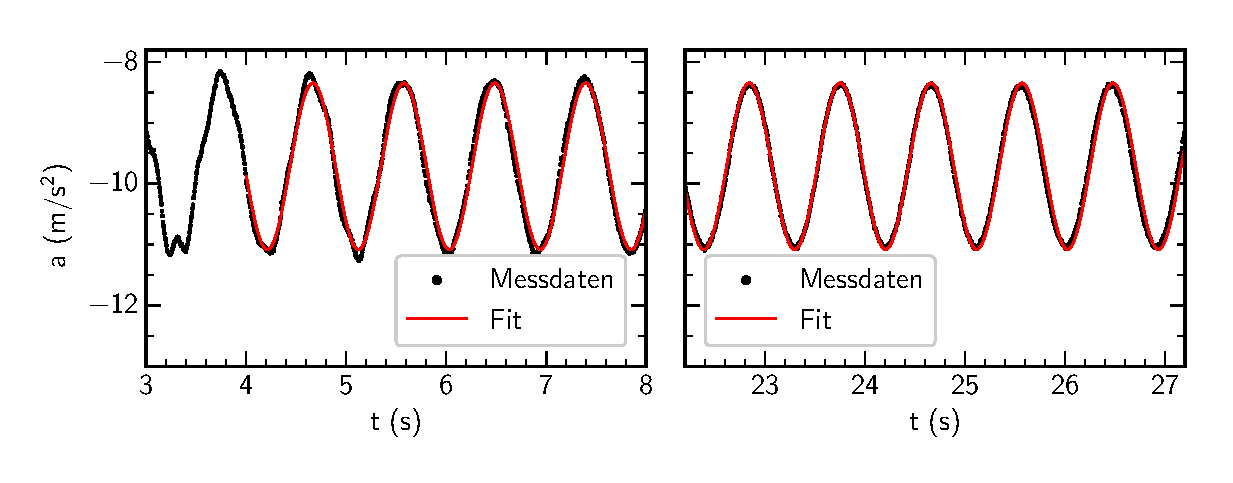
\includegraphics[width=\textwidth]{Feder1.eps}
	\caption[Oszillation mit einer Feder]{Die Beschleunigung wurde auf die Zeit aufgetragen und eine durchgehende Sinuskurve in Rot wurde an die Daten ab \( t = 4 \unit{s} \) (bis \( t = 27 \unit{s} \)) angepasst. Dargestellt werden aber nur ersten 5 Sekunden (links) beziehungsweise letzten 5 Sekunden (rechts). Die Fehlerbalken der Daten sind zu klein, um sie auszumachen und werden daher nicht eingetragen.}
	\label{fig:sine}
\end{figure}
	
Aus dem Fit lässt sich direkt die Winkelfrequenz \( \omega \) herauslesen. Aus dieser kann man wiederum mit \autoref{eqn:T} die Schwingungsdauer berechnen. In \autoref{table:2} sind charakteristische Eigenschaften der Schwingung, wie die Kreisfrequenz oder die Masse, eingetragen. 
	
\begin{center}
	\captionaboveof{table}[Messdaten zur Oszillation einer Feder]{Gemessene Masse, Schwingungsdauer, Winkelfrequenz und Federkonstante der drei Versuche.}
	\begin{tabular}{@{\extracolsep{5mm}} 
			r
			S[table-format=1.3(1)]
			S[table-format=1.3(1)]
			S[table-format=1.3(1)]
		}
		\toprule
		\makecell[t]{}
		&   {\makecell[t]{Versuch 1}}
		&   {\makecell[t]{Versuch 2}}
		&   {\makecell[t]{Versuch 3}}\\
		\midrule
		\( m \unit{(kg)}\) & 0.202(2) & 0.286(3) & 0.400(7) \\
		\( \tilde{m} \unit{(\sqrt{1/kg})} \) & 2.223(10) & 1.8698(99) & 1.580(15) \\
		\( T \unit{(s)} \) & 0.749(2) & 0.909(5) & 1.063(10) \\
		$\omega \unit{(1/s)}$ & 8.39(2) & 6.91(4) & 5.91(6) \\
		\( k \unit{(N/m)} \) & 14.24(15) & 13.7(2) & 14.0(4) \\
		\bottomrule
	\end{tabular}
	\label{table:2}
\end{center}

Das Modell des harmonischen Oszillators (Siehe \autoref{eqn:omega}) stellt einen linearen Zusammenhang zwischen \( \omega \) und der Wurzel des Kehrwerts der Masse \( \tilde{m} \) her mit\( \sqrt{k} \) als Proportionalitätskonstante. Dies wird in \autoref{fig:k1} anhand der in \autoref{table:1} angegebenen Werten illustriert. Zusätzlich zu den drei Datenpunkten wurde eine Gerade, wie sie das Modell vorhersagt, angepasst, wodurch man für die Steigung der linearen Funktion \( \sqrt{k} = 3.74(2) \unit{\sqrt{kg / s^2}} \) erhält. Nachdem wir kein Indiz dafür haben, dass die Gerade die Ordinate nicht im Ursprung schneidet, wurde der Fit gezielt mit nur einem Parameter (der Steigung) durchgeführt, um die Anzahl der Freiheitsgrade von 1 auf 2 zu erhöhen. 

\begin{figure}[H]
	\centering
	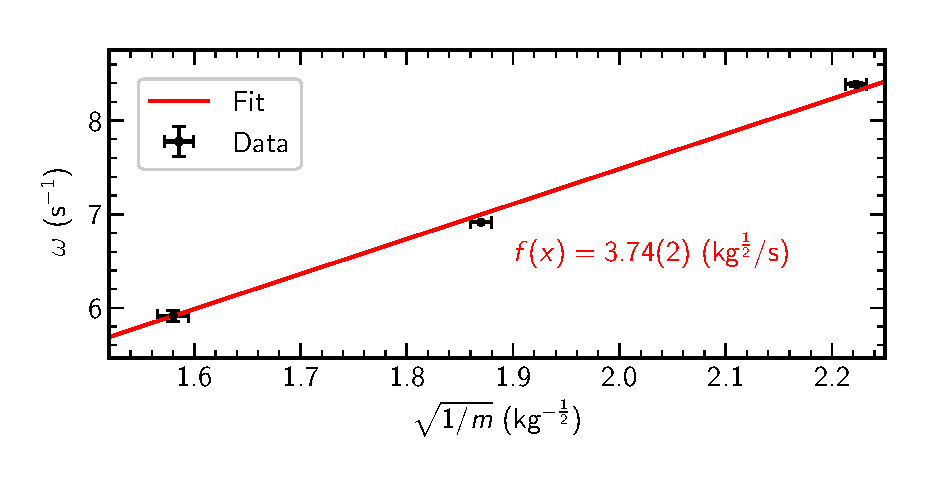
\includegraphics[width=\textwidth]{k1.eps}
	\caption[Zusammenhang zwischen \( \omega \) und \( \tilde{m} \)]{Winkelfrequenz für drei unterschiedliche Massen. In rot wurde eine lineare Funktion durch den Ursprung angepasst. Die Fehlerbalken stellen den $1\sigma$ Fehler dar; die Unsicherheit in \( \omega \) ist so gering, dass sie kaum sichtbar ist.}
	\label{fig:k1}
\end{figure}

\chapter{Diskussion und Schlussfolgerung}
\label{chap:schlussfolgerung}

%Abschließend


%Literaturverzeichnis
\bibliographystyle{unsrtdin}
\bibliography{Literatur}

\end{document}
